\chapter{Related Work} \label{chap:relatedwork}

This chapter describes existing systems used to create secure workstations. We provide a brief summary of each of the following systems and analyze its limitations.

\paragraph{Qubes OS:} Qubes OS is an operating system which uses virtualization to provide isolation. It provides features such as the ability to create tiered VMs based on security levels, firewall policies to restrict network traffic in respective tiers, and a secure user interface implementation. Quboid uses Qubes OS as its base to preset a secure workstation.

\paragraph{Bromium:} Bromium is a similar system to Qubes OS which uses a technology called micro-virtualization to provide similar isolation guarantees while retaining the performance benefits of traditional OS processes. The idea of running each application in a separate virtual machine is used in the design of Quboid.

\paragraph{Google Chrome Browser:} The Google Chrome Browser uses isolation techniques to execute tabs in a sandbox. This largely prevents attacks that take advantage of browser exploits. Quboid has a similar goal to Chrome Browser - to provide users the ability to browse the web safely.

\paragraph{Spam Filters:} Since most cyberattacks begin with a phishing email, we analyze the spam-filtering systems used by Gmail, a popular email provider. We analyze the effectiveness of the parameters used by the Gmail filters and its limitations.

\paragraph{EROS Trusted Window System (EWS):} The user interface is another system which phishing attacks take advantage of. EWS is a system which uses the concept of trusted path for user interaction to provide a trusted window system.

\section{Qubes OS} \label{section-qubes-os}

Qubes OS is a security oriented operating system based on Xen hypervisor \cite{xen}. It uses virtualization to provide isolation among applications running in different security levels. Users have the ability to create virtual machines and designate them with different security levels for use with different applications. For example, banking and credit card applications can reside in a trusted VM whereas general everyday browsing can occur in an untrusted VM. The Qubes OS interface is a GUI running in Xen's dom0, the built-in trusted VM which is allowed to perform management operations on the hypervisor. Qubes OS provides several features to ensure that dom0 is never compromised even if one of the virtual machines gets compromised.

The following subsections describe the isolation guarantees provided through virtualization, firewall policies for the VMs and the Qubes user interface:

\subsection{Isolation using Virtualization}

The virtual machines in Qubes OS run complete operating systems. However, they all share the same root filesystem which is read-only. Any modifications done by the VMs to the root filesystem are performed in-memory and are rolled back when the VM is shut down. Additionally, each VM also has a personalized home filesystem which stores persistent data.

Having such a strict isolation between different VMs provides better security but also decreases usability. Qubes OS has the following features to overcome this limitation:

\paragraph{Clipboard Sharing} Qubes OS lets VMs copy and paste data to and from their own clipboards through the use of shared memory between VMs. The dom0 is not involved in the data exchange which reduces the attack surface.

\paragraph{Disposable VMs} A user may want to run an application just once in a separate isolated VM. In a normal workflow, the user will have to create a new VM with an operating system, run the application in it, and then delete the VM. To simplify this workflow, Qubes OS has a feature called Disposable VMs. A disposable VM runs like a normal VM but has an ephemeral hard disk. It can be booted up within seconds to run an application and then destroyed. It is based on an existing template so the user does not have to reinstall the operating system every time a new disposable VM is created.

\subsection{Firewall Policies}

Qubes OS implements strict network isolation. No inter-VM communication is possible unless the user explicitly modifies the configuration. Network traffic from each VM is routed through an intermediate VM called the FirewallVM. The FirewallVM runs a traditional port-based firewall called {\tt iptables}. Users can change the firewall policies through the VM management interface. However, these policies are limited to allowing or denying traffic to and from a specific IP address and/or port.

The management VM, dom0, is completely isolated and has no network access. This ensures any outside attacks are not able to target and compromise dom0. If dom0 requires network access, for example when performing an update, the necessary files are downloaded into a separate VM, checked for integrity and then copied over to dom0 through the use of shared memory.

\subsection{User Interface}

The user interface is an important aspect to focus on to combat phishing attacks. Most phishing attacks pretend to be a trusted website in order to trick the user into entering their credentials and other sensitive information. Qubes OS makes sure that all applications running in different security levels appear visually separate from each other through the use of window border colors. For example, the trusted VM can have a green border color whereas the untrusted VM can have a red border color. The users must ensure that they only enter their information in the trusted VM when they see a green border color around the application. The user is also allowed to rename the VMs which provides an additional method to verify that they are entering their information in the correct VM. Figure~\ref{fig:qubes-screenshot} shows a screenshot of the Qubes OS user interface.

\afterpage{\clearpage
\begin{figure}[p]
\centering
    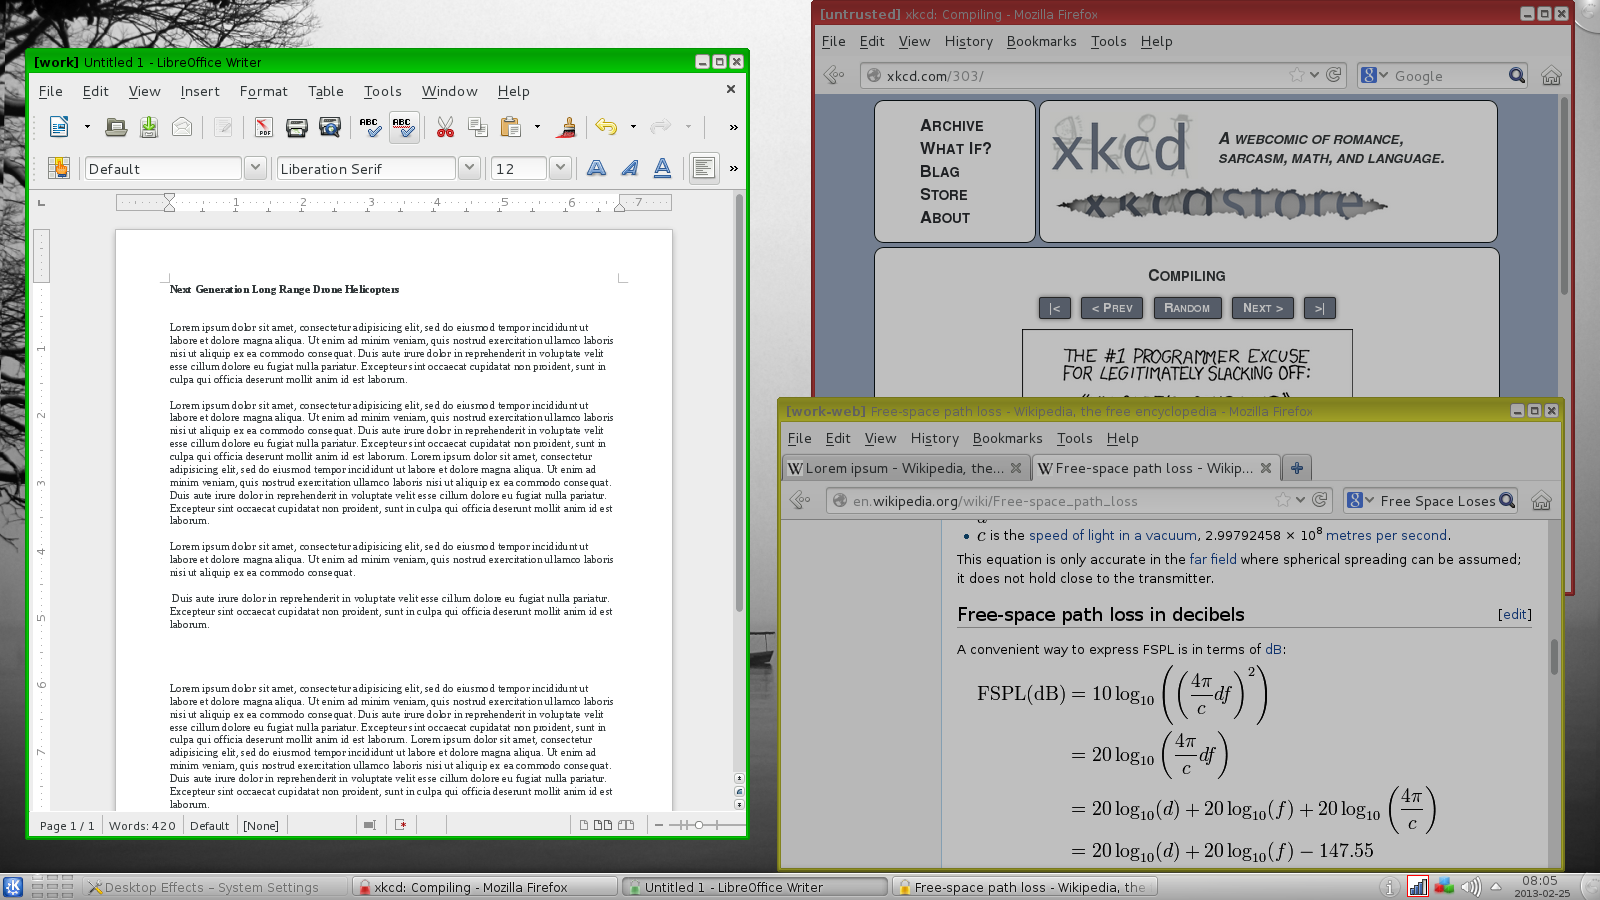
\includegraphics[width=1.0\textwidth]{qubes-screenshot.png}
    \caption{This screenshot shows the user interface of Qubes OS. Each of the applications is running in a separate virtual machine. The user has labelled the virtual machines as [work], [work-web] and [untrusted], and have given appropriate border colors to visually differentiate the virtual machines.}
   \label{fig:qubes-screenshot}
\end{figure}
\clearpage
}

\subsection{Limitations}

Although Qubes OS provides strong security guarantees, it has its limitations for defending against phishing attacks.

\paragraph{No support for advanced firewall rules:} The firewall is only able to filter based on IP and port. Advanced filters based on hostnames are unavailable. This is specially important because a user may want to designate a VM as their bank VM and have firewall rules prohibiting any traffic except to their bank. If the bank's website changes IP addresses, for example via a load balancer, an IP and port based firewall proves insufficient. The Site Aggregate Isolation policy described in this thesis requires the use of advanced filter rules.

\paragraph{Ambiguity in the user interface:} The border color and custom naming strategy is not enough to defend against some phishing attacks. Qubes OS uses a stacking window manager. It can have multiple resizable windows which can be stacked on top of each other. It is possible for an untrusted VM window to pretend to contain a trusted VM inside its bounds and can trick the user into entering their credentials into the untrusted VM.

\section{Bromium}

Bromium \cite{bromium} is a virtualization-based system similar to Qubes OS in several aspects. It uses virtualization to run applications in separate virtual machines, similar to Qubes OS. One major difference is instead of running a full operating system in a VM, it uses a technology called micro-virtualization. Micro-VMs are lightweight processes which share a lot of resources with the hypervisor while still retaining the isolation guarantees obtained by running full virtual machines. This allows users to quickly launch applications in new virtual machines without going through an OS boot cycle.

Another feature provided by Bromium is the ability to preform post-exploitation analysis. If the system determines that a possible attack is underway, it notifies the user and allows the user to perform analysis on the attack. While attacks are still possible, the damage is contained to the virtual machine where the infected application resides. It is unable to compromise the rest of the system.

The ability to run application in separate VMs is specially effective against ransomware attacks. In such types of attacks, the malicious software encrypts the whole hard drive, sends the decryption keys to the attackers, and deletes those keys from the local system. The only way to recover the data then is to pay the attackers a sum of money in order to retrieve the decryption keys. Figure~\ref{fig:wannacry} shows a screenshot of the prompt shown after the WannaCry ransomware has finished the encryption. This was a recent ransomware attack which compromised several U.K. hospitals.

\afterpage{\clearpage
\begin{figure}[p]
\centering
    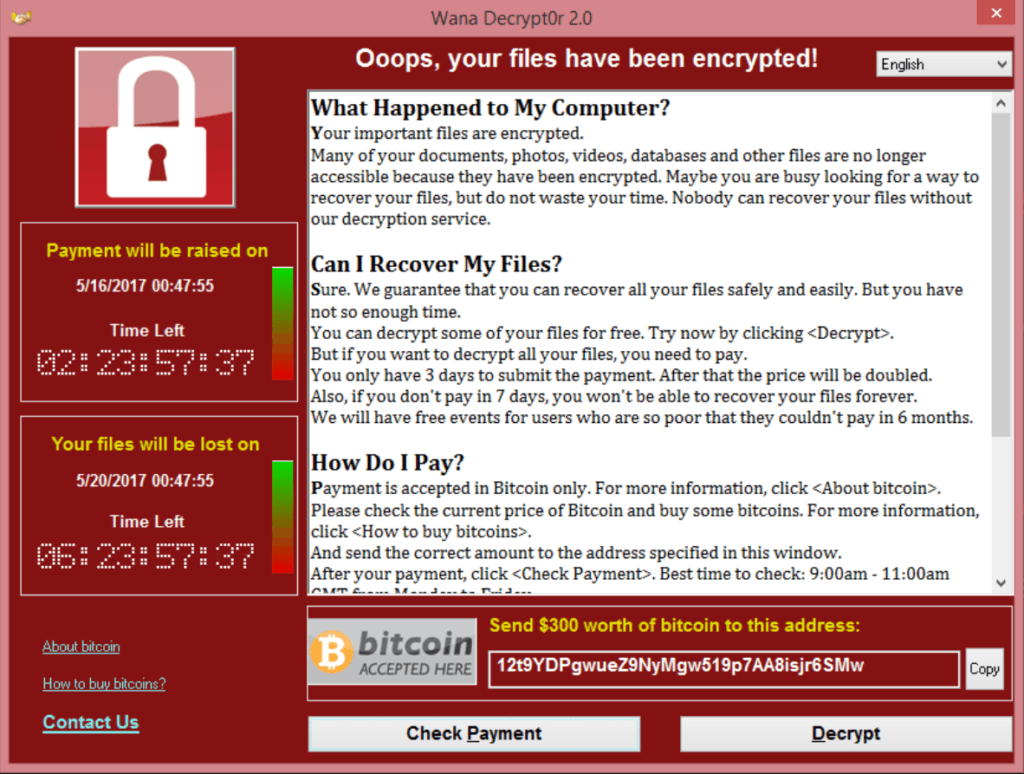
\includegraphics[width=1.0\textwidth]{wannacry.png}
    \caption{This screenshot shows the prompt shown after the WannaCry ransomware has finished encryption of the whole hard disk. The attack uses a bug in the OS to compromise the whole system. It then encrypts the hard disk, sends the decryption keys to the attackers and then deletes those keys from the local system. The only way to recover the keys is by paying the attacker \$300 via Bitcoin and hoping to re-obtain the decryption keys.}
   \label{fig:wannacry}
\end{figure}
\clearpage}

If a ransomware was to attack a system running Bromium, it will only have access to the hard disk associated with the virtual machine where the application is running. Once the application is closed, the virtual machine is shutdown destroying all traces of the attack. 

Qubes OS also shares similar advantages, however, it is possible to have multiple applications installed in the same virtual machine. The ransomware attack could still
encrypt the contents of the other applications. Bromium provides a stronger security guarantee by executing each application in its own virtual machine.

\subsection{Limitations}

Although Bromium defends against phishing attacks that lead to downloading malicious software, it does not defend against phishing attacks that are designed to steal user information. Bromium provides no defense against attacks that are designed to trick the user into entering sensitive information and steal their details, for example, a website can still display a fake login form and Bromium will not give any indication that something is wrong.

\section{Google Chrome Browser}

The Google Chrome Browser is a popular modern-day browser. It has been the leader of the browser market share for more than a year, surpassing Microsoft Internet Explorer in March 2016 in the desktop browser market share \cite{marketsharereport}. It provides a simple user interface and several features to increase the usability and security of the browser. However, the highlighting feature of Chrome is its sandbox.

The Chrome sandbox \cite{chromesandbox} is a mechanism to provide guarantees on what a piece of code can and cannot do. The rendering engine of each tab is run in a sandbox. The sandbox leverages existing operating system mechanisms to restrict the privileges the code has. It forbids access to the file system, display, clipboard, operating system hooks, etc. The rendering engine draws onto an off-screen buffer which the browser then displays to the user.

The threat model for the sandbox operates under the assumption that the code executing is malicious and the sandbox has been compromised. Thus, a lot of features are focused on making sure the code cannot take advantage of browser bugs to compromise the system.

\namesecureworkstation/ uses similar ideas as Google Chrome, for example, executing code from different websites in isolation from each other. The virtual machine in \namesecureworkstation/ serves the same purpose as the sandbox serves in Chrome. Virtualization is a step forward in providing isolation in additional contexts, such as the ability to execute malicious executable file in a contained environment.

\subsection{Limitations}

The Chrome sandbox contains any code running within a tab in a sandbox. However, it does not prevent any downloaded code to execute in an isolated environment. If the user downloads a malicious file, it will still be able to compromise the entire system.

Additionally, Chrome does not have mechanisms to prevent phishing attacks. Similar to most other browsers, it warns the user about inconsistencies in the browser SSL/TLS certificates. It also maintains a blacklist of malicious websites and warns the user when navigating to such websites. However, any website not in the blacklist or with valid certificates can still be able to trick the user into compromising their credentials.

\section{Spam Filters}

A lot of phishing attacks use emails to spread. A recent attack \cite{google-docs-phishing} started with users clicking on a phishing email which pretended to contain a link to a shared document on Google Drive. The attackers were then able to obtain the user's Gmail authentication token which was used to automatically forward the email to everyone on the user's contacts list. Fortunately, most of the email providers implement some sort of spam filtering before the email reaches the user's inbox to prevent such sort of attacks.

For example, Gmail uses the following list \cite{gmail-spam-filter-list} to determine when emails should be automatically marked as spam. We only list the parameters which are relevant for defending against phishing attacks:

\paragraph{Spoofed email addresses:} If the sender's email address is very similar to a known email address, for example {\tt contact@company.org} and {\tt c0ntact@company.org}, users may mistake the latter to also be a legitimate source. Gmail recognizes such spoofs and automatically marks them as spam.

\paragraph{Known phishing scams:} Gmail lets users mark emails as phishing. If enough users mark similar looking emails as phishing, it is an indication that any such future emails should be automatically marked as spam. However, this strategy fails if the phishing scam is new and not enough feedback has been gathered from user reports.

\paragraph{Messages from unconfirmed sender:} If Gmail is unable to verify that the email was sent from the source it claimed to be sent from, it is marked as spam. This strategy is helpful when attackers try to send emails with legitimate source email address from unauthorized email servers, for example, public SMTP servers.

\subsection{Limitations}

Although these strategies are helpful against most phishing attacks, some phishing email may still end up in user's inbox. Emails that originate from legitimate email addresses, or attacks which are fairly new and haven't been flagged yet can bypass these mechanisms.

\section{EROS Trusted Window System}

The EROS Window System (EWS) \cite{eros} is a window system which provides strict access controls to the user and claims to not introduce any new covert channels in the display system. It is a minimal implementation of a secure window system and is under 4,500 lines of code. The system provides isolation between applications and allows no communication between them unless the user has specifically authorized so.

The system makes sure that any communication between application should only be allowed if it can be traced by back to an authorizing user action. This system also addresses some part of user interface security. In particular, it provides a small code footprint which is easy to very for security bugs. It addresses partially the issue of user interface ambiguity by using different brightness for active and inactive windows.

An important property that this system provides is the principle of isolation and restricted communication. Client sessions operate in isolation of each other, no session can affect or observe state from other sessions. Additionally, the display server restricts the kind of communication that can place between processes. The design of \namesecureworkstation/ applies the idea of isolation and restricted communication to different websites i.e. different websites must not share state and there must be restricted communication between them.

\subsection{Limitations}

EWS is a not complete secure workstation solution. It addresses the issue of security between different processes on the system. However, security while web browsing requires a completely different solution. Several forms of phishing attacks don't rely on faking windows and window actions. We can however take inspiration from the ideas of EWS such as isolation and restricted communication to design a secure workstation.
